% !TEX root = epifanov_solid_state_physics.tex
%!TEX TS-program = pdflatex
%!TEX encoding = UTF-8 Unicode

\appendix

\chapter*{APPENDICES}\label{chap:A}
\addcontentsline{toc}{chapter}{APPENDICES}
\chaptermark{APPENDICES}
\renewcommand{\thechapter}{A}
\setcounter{section}{0}
\renewcommand{\thesection}{\thechapter.\arabic{section}}
% \setcounter{theorem}{0}
% \renewcommand{\thetheorem}{\thechapter.\arabic{theorem}}
\setcounter{equation}{0}
\renewcommand{\theequation}{\thechapter.\arabic{equation}}
\setcounter{figure}{0}
\renewcommand{\thefigure}{\thechapter.\arabic{figure}}
\setcounter{table}{0}
\renewcommand{\thetable}{\thechapter.\arabic{table}}

\section{Derivation of the Maxwell-Boltzmann distribution function}\label{sec:A_I}

To obtain expression \eqref{eq:3_25}, consider a collision of two particles one of which is in a state with the energy $E_1$ and the other in a state with the energy $E_2$. After the collision the particles will go over to states with energies $E_3$ and $E_4$, respectively. Let us define the term \textit{reverse collision} as a collision that returns the particles to the initial states with the energies $E_1$ and $E_2$. Thus, we shall consider collisions of two types:
\begin{align*}
    (E_1, E_2) &\to (E_3, E_4)\quad\text{(direct)}\\
    (E_3, E_4) &\to (E_1, E_2).\quad\text{(inverse)}
\end{align*}

The rate of direct collisions $\ab{Q}{d}$ is proportional to the average number of particles in the initial state, that is $f(E_1)$ and $f(E_2)$, and is independent of the number of particles in the final state because the gas is nondegenerate:
\begin{equation}\label{eq:A_1}
    \ab{Q}{d} = c f(E_1) f(E_2),
\end{equation}

\noindent
where $c$ is a proportionality factor.

The number of reverse collisions is proportional to $f(E_3) f(E_4)$:
\begin{equation}\label{eq:A_2}
    \ab{Q}{r} = c f(E_3) f(E_4).
\end{equation}

\noindent
In the state of thermodynamic equilibrium $\ab{Q}{d}$ should be equal to $\ab{Q}{r}$:
\begin{equation}\label{eq:A_3}
    f(E_1) f(E_2) = f(E_3) f(E_4).
\end{equation}

\noindent
Making use of the energy conservation law, $E_1+E_2=E_3+E_4$, we may rewrite the expression in the form:
\begin{equation}\label{eq:A_4}
    f(E_1) f(E_2) = f(E_3) f(E_1 + E_2 - E_3).
\end{equation}

\noindent
Note that $E_1$, $E_2$, $E_3$ must be regarded as independent quantities. Taking the logarithm of both sides of \eqn{A_4}, we obtain
\begin{equation}\label{eq:A_5}
    \ln\bracket{f(E_1) f(E_2)} = \ln\bracket{f(E_3) f(E_1 + E_2 - E_3)}.
\end{equation}

Differentiate this sum with respect to $E_1$. Since $E_2$ and $E_3$ are independent of $E_1$, they may be assumed to be constant. Then,
\begin{equation}\label{eq:A_6}
    \frac{1}{f(E_1)} \diff{f(E_1)}{E_1} = \frac{1}{f(E_1 + E_2 - E_3)} \diff{f(E_1 + E_2 - E_3)}{f(E_1 + E_2 - E_3)} \diff{f(E_1 + E_2 - E_3)}{E_1}.
\end{equation}

Since $\diffin{f(E_1+E_2-E_3)}{E_1}=1$, it follows that
\begin{equation}\label{eq:A_7}
    \frac{1}{f(E_1)} \diff{f(E_1)}{E_1} = \frac{1}{f(E_1 + E_2 - E_3)} \diff{f(E_1 + E_2 - E_3)}{f(E_1 + E_2 - E_3)}.
\end{equation}

\noindent
Differentiate \eqn{A_5} with respect to $E_2$:
\begin{equation}\label{eq:A_8}
    \frac{1}{f(E_2)} \diff{f(E_2)}{E_2} = \frac{1}{f(E_1 + E_2 - E_3)} \diff{f(E_1 + E_2 - E_3)}{f(E_1 + E_2 - E_3)}.
\end{equation}

\noindent
Comparing \eqn{A_7} with \eqn{A_8}, we obtain
\begin{equation}\label{eq:A_9}
    \frac{1}{f(E_1)} \diff{f(E_1)}{E_1} = \frac{1}{f(E_2)} \diff{f(E_2)}{E_2}.
\end{equation}

The left-hand side of \eqn{A_9} is independent of $E_2$, the right-hand side is independent of $E_1$; therefore, each of them is equal to some constant independent of the particles' energy. Denote it by $\beta$. Then, we may rewrite \eqn{A_9} as follows:
\begin{equation}\label{eq:A_10}
    \frac{1}{f(E)} \diff{f(E)}{E} = \beta.
\end{equation}

\noindent
Integrating \eqn{A_10}, we obtain
\begin{equation}\label{eq:A_11}
    f(E) = A\, e^{\beta E},
\end{equation}

\noindent
where $A$ is the integration constant. Experiment shows that
\begin{equation}\label{eq:A_12}
    \beta = -\frac{1}{\ab{k}{B}T},\quad A\, e^{\mu/(\ab{k}{B}T)}.
\end{equation}

Substituting \eqn{A_12} into \eqn{A_11}, we finally get
\begin{equation}\label{eq:A_13}
    \ab{f}{M}(E) = e^{\mu/(\ab{k}{B}T)}\, e^{-E/(\ab{k}{B}T)}.
\end{equation}

\section{Derivation of the Fermi-Dirac distribution function}\label{sec:A_II}

Consider, as we did in Appendix \ref{sec:A_I}, the direct and reverse particle collisions. Recall that in the case of a nondegenerate gas, the rate of collisions was independent of the number of particles in the final stages and was entirely determined by the number of particles in the initial stages. The situation in the case of a degenerate fermion gas is a different one: if a state is already occupied, it cannot accept another fermion and the collision will not take place. For this reason, in the case of a degenerate fermion gas, the rate of collisions is proportional not only to the average number of particles in the initial states but to the average number of vacant states with the energies $E_3$ and $E_4$ as well.

Since $\ab{f}{F}(E)$ expresses the probability for the state with the energy $E$ to be occupied, $1-\ab{f}{F}(E)$ expresses the probability for it to be vacant. Therefore, the average numbers of vacant states with the energies $E_3$ and $E_k$ are $1-\ab{f}{F}(E_3)$ and $1-\ab{f}{F}(E_4)$, respectively.
Accordingly, the rates of direct and reverse collisions are:
\begin{align}
    \ab{Q}{d} &= c\ab{f}{F}(E_1)\ab{f}{F}(E_2) \bracket{1-\ab{f}{F}(E_3)} \bracket{1-\ab{f}{F}(E_4)}, \label{eq:II_1}\\
    \ab{Q}{r} &= c\ab{f}{F}(E_3)\ab{f}{F}(E_4) \bracket{1-\ab{f}{F}(E_1)} \bracket{1-\ab{f}{F}(E_2)}. \label{eq:II_2}
\end{align}

\noindent
In the state of thermal equilibrium
\begin{align}
    \ab{f}{F}(E_1) \ab{f}{F}(E_2) &\bracket{1-\ab{f}{F}(E_3)} \bracket{1-\ab{f}{F}(E_4)}\nonumber\\
    & = \ab{f}{F}(E_3)\ab{f}{F}(E_4) \bracket{1-\ab{f}{F}(E_1)} \bracket{1-\ab{f}{F}(E_2)}.\label{eq:II_3}
\end{align}

\noindent
Dividing both sides of \eqn{II_3} by $\ab{f}{F}(E_1) \ab{f}{F}(E_2) \ab{f}{F}(E_3)\ab{f}{F}(E_4)$, we
obtain
\begin{equation}\label{eq:II_4}
    \bracket{\frac{1}{\ab{f}{F}(E_1)} - 1} \bracket{\frac{1}{\ab{f}{F}(E_2)} - 1} = \bracket{\frac{1}{\ab{f}{F}(E_3)} - 1} \bracket{\frac{1}{\ab{f}{F}(E_4)} - 1}.
\end{equation}

\noindent
Comparing \eqn{II_4} with \eqn{A_4}, one may easily see that the function $1/\ab{f}{F}(E)-1$, for a degenerate fermion gas, satisfies the same condition as is satisfied by the function $\ab{f}{F}(E)$ in the case of a nondegenerate gas. This makes it possible to use the result \eqn{A_10}, which in this case takes the form
\begin{equation}\label{eq:II_5}
    \bracket{\frac{1}{\ab{f}{F}(E)} - 1}^{-1} \diff{}{E}\bracket{\frac{1}{\ab{f}{F}(E)} - 1} = \gamma,
\end{equation}

\noindent
where $\gamma$ is a constant. Integrating \eqn{II_5}, we obtain
\begin{equation}\label{eq:II_6}
    \frac{1}{\ab{f}{F}(E)} = B\, e^{\gamma E},
\end{equation}

\noindent
where $B$ is the integration constant.

The following considerations may be of use to estimate the constants $\gamma$ and $B$. When the condition $\ab{f}{F}(E)\ll 1$ is satisfied, the fermion gas becomes nondegenerate. For such a gas, we can neglect unity in the left-hand side of \eqn{II_6} and rewrite the expression in the form:
\begin{equation}\label{eq:II_7}
    \ab{f}{F}(E) = B^{-1}\, e^{-\gamma E}.
\end{equation}

\noindent
Comparing \eqn{II_7} with \eqn{A_2}, and keeping in mind \eqn{A_12}, we obtain:
\begin{equation}\label{eq:II_8}
    B = A^{-1} = e^{-\mu/(\ab{k}{B}T)},\quad \gamma = -\beta = \frac{1}{\ab{k}{B}T}.
\end{equation}

\noindent
Substituting into \eqn{II_6}, we finally obtain
\begin{equation}\label{eq:II_9}
    \ab{f}{F}(E) = \frac{1}{e^{(E-\mu)/(\ab{k}{B}T)} + 1}.
\end{equation}

\section{Derivation of the Bose-Einstein distribution function}\label{sec:A_III}

In contrast to fermions, bosons can occupy both vacant states and states already occupied by other bosons and they do it the more readily the greater is the occupancy of the states. Therefore, the rate of direct collisions $E_1\to E_3$, $E_2\to E_4$ will be the greater, the greater the numbers of particles in the initial states $\ab{f}{Bose}(E_1)$ and $\ab{f}{Bose}(E_2)$ and the higher the occupancy of the final states $\ab{f}{Bose}(E_3)$ and $\ab{f}{Bose}(E_4)$:
\begin{equation}\label{eq:III_1}
    \ab{Q}{d} = c \ab{f}{Bose}(E_1) \ab{f}{Bose}(E_2) \bracket{1 + \ab{f}{Bose}(E_3)} \bracket{1 + \ab{f}{Bose}(E_4)}.
\end{equation}

The units in the brackets take account of the bosons' ability to go over not only to occupied states but to vacant states, for which $\ab{f}{Bose}(E_3)=\ab{f}{Bose}(E_4)=0$, as well. For $\ab{f}{Bose}(E)\gg 1$ (the condition of nondegeneracy), the expression in the brackets in \eqn{III_1} becomes unity and $\ab{Q}{d}$ becomes equal to the rate of direct collisions for the particles of a nondegenerate gas. For the rate of reverse collisions $E_3\to E_1$, $E_4\to E_2$, we obtain
\begin{equation}\label{eq:III_2}
    \ab{Q}{r} = c \ab{f}{Bose}(E_3) \ab{f}{Bose}(E_4) \bracket{1 + \ab{f}{Bose}(E_1)} \bracket{1 + \ab{f}{Bose}(E_2)}.
\end{equation}

In the state of equilibrium $\ab{Q}{d}=\ab{Q}{r}$:
\begin{align}
    \ab{f}{Bose}(E_1) &\ab{f}{Bose}(E_2) \bracket{1 + \ab{f}{Bose}(E_3)} \bracket{1 + \ab{f}{Bose}(E_4)} \nonumber\\
    & = \ab{f}{Bose}(E_3) \ab{f}{Bose}(E_4) \bracket{1 + \ab{f}{Bose}(E_1)} \bracket{1 + \ab{f}{Bose}(E_2)}. \label{eq:III_3}
\end{align}

\noindent
Dividing this expression by $\ab{f}{Bose}(E_1) \ab{f}{Bose}(E_2) \ab{f}{Bose}(E_3) \ab{f}{Bose}(E_4)$, we obtain
\begin{equation}\label{eq:III_4}
    \bracket{\frac{1}{\ab{f}{Bose}(E_1)} + 1} \bracket{\frac{1}{\ab{f}{Bose}(E_2)} + 1} = \bracket{\frac{1}{\ab{f}{Bose}(E_3)} + 1} \bracket{\frac{1}{\ab{f}{Bose}(E_4)} + 1}.
\end{equation}

\noindent
A comparison between \eqns{III_4}{A_3} shows that the function $1/\ab{f}{Bose}(E_1) + 1$ for bosons, satisfies the same equation as the function $f(E)$ for a nondegenerate gas. Therefore, we may make use of the result \eqref{eq:A_10} writing it for bosons in the form
\begin{equation}\label{eq:III_5}
    \frac{1}{\bracket{\ab{f}{Bose}(E)^{-1} + 1}} \diff{}{E} \bracket{\frac{1}{\ab{f}{Bose}(E)} + 1} = \gamma.
\end{equation}

\noindent
Integrating \eqn{III_5}, we obtain
\begin{equation}\label{eq:III_6}
    \frac{1}{\ab{f}{Bose}(E)} + 1 = B\, e^{\gamma E}.
\end{equation}

\noindent
The values of the constants $\gamma$ and $B$ that enter this expression are the same as in the case of the degenerate fermion gas:
\begin{equation}\label{eq:III_7}
    \gamma = \frac{1}{\ab{k}{B}T},\quad B = e^{-\mu/(\ab{k}{B}T)}.
\end{equation}

\noindent
Therefore,
\begin{equation}\label{eq:III_8}
    \ab{f}{Bose}(E) = \frac{1}{e^{(E-\mu) / (\ab{k}{B}T)} - 1}.
\end{equation}

\section{Tables}\label{sec:A_IV}

\begin{table}[h]
	\renewcommand{\arraystretch}{1.2}
	\caption{}
	\vspace{-0.6cm}
	\label{table:A_1}
	\begin{center}\resizebox{0.9\linewidth}{!}{
		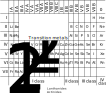
\includegraphics[scale=0.8]{figures/appendix/fig_app_table_1.pdf}
	}\end{center}
\end{table}

\vspace*{-1cm}

\begin{table}[!h]
	\renewcommand{\arraystretch}{1.2}
	\caption{}
	\vspace{-0.6cm}
	\label{table:A_2}
	\begin{center}\resizebox{0.9\linewidth}{!}{
		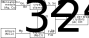
\includegraphics[scale=0.85]{figures/appendix/fig_app_table_2.pdf}
	}\end{center}
\end{table}
